\begin{figure}[htbp]
	% Partly taken from http://www.texample.net/tikz/examples/convolution-of-two-functions/
	\centering
	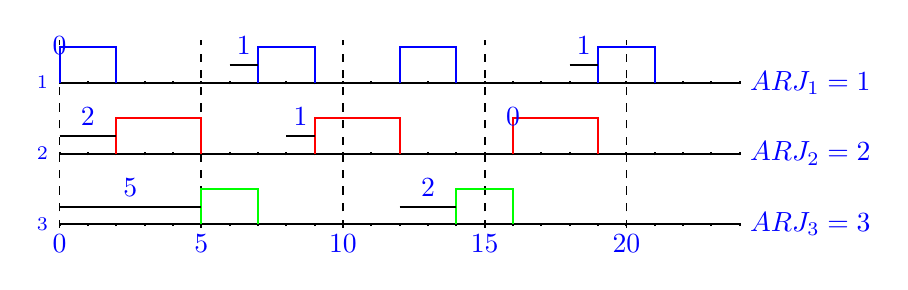
\begin{tikzpicture}[
		scale=0.09,
		line width=0.25mm,
		every node/.style={scale=1, text=blue},
		major tick/.style={semithick, dashed},
		x tick label/.style={anchor=north, minimum width=5mm},
		task1/.style={blue},
		task2/.style={red},
		task3/.style={green},
		desc/.style={anchor=east},
		arj/.style={anchor=west},
		desc2/.style={anchor=south}
		]

	% 24 96
	% Task 3
	\draw (0, 0) -- (96, 0);
	\node[desc] at (0, 0) {$\uptau_3$};
	
	% Task 2
	\draw (0, 10) -- (96, 10);
	\node[desc] at (0, 10) {$\uptau_2$};	

	% Task 1
	\draw (0, 20) -- (96, 20);
	\node[desc] at (0, 20) {$\uptau_1$};

	
	% Small ticks
	\foreach \x in {0, 4,...,96}{
		\draw (\x, -0.25) -- (\x, 0.25);
		\draw (\x, 19.75) -- (\x, 20.25);
		\draw (\x, 9.75) -- (\x, 10.25);
	}
	
	% Major ticks with label
	\foreach \x/\label in {0, 20,...,96}{		
		\draw[major tick] (\x, -0.5) -- (\x, 26);
	}
	
	\node[x tick label] at (0, 0) {0};
	\node[x tick label] at (20, 0) {5};
	\node[x tick label] at (40, 0) {10}; 
	\node[x tick label] at (60, 0) {15};
	\node[x tick label] at (80, 0) {20};
	
	% Draw all
	\draw[task1] (   0, 20) -- (   0, 25) -- ( 2*4, 25) -- ( 2*4, 20);
	\draw[task2] ( 2*4, 10) -- ( 2*4, 15) -- ( 5*4, 15) -- ( 5*4, 10);
	\draw[task3] ( 5*4,  0) -- ( 5*4,  5) -- ( 7*4,  5) -- ( 7*4,  0);
	\draw[task1] ( 7*4, 20) -- ( 7*4, 25) -- ( 9*4, 25) -- ( 9*4, 20);
	\draw[task2] ( 9*4, 10) -- ( 9*4, 15) -- (12*4, 15) -- (12*4, 10);
	\draw[task1] (12*4, 20) -- (12*4, 25) -- (14*4, 25) -- (14*4, 20);
	\draw[task3] (14*4,  0) -- (14*4,  5) -- (16*4,  5) -- (16*4,  0);
	\draw[task2] (16*4, 10) -- (16*4, 15) -- (19*4, 15) -- (19*4, 10);
	\draw[task1] (19*4, 20) -- (19*4, 25) -- (21*4, 25) -- (21*4, 20);

	% Task 1
	\node[desc2] at      (     0, 22.5) {0};
	\draw ( 6*4,22.5) -- (   7*4, 22.5);	
	\node[desc2] at      ( 6.5*4, 22.5) {1};
	\draw (18*4,22.5) -- (  19*4, 22.5);	
	\node[desc2] at      (18.5*4, 22.5) {1};
	\node[arj] at (96, 20)  {$ARJ_1=1$};
	
	% Task 2 ARJ
	\draw (   0,12.5) -- (  2*4, 12.5);
	\node[desc2] at      (  1*4, 12.5) {2};
	\draw ( 8*4,12.5) -- (  9*4, 12.5);
	\node[desc2] at      (8.5*4, 12.5) {1};
	\node[desc2] at      ( 16*4, 12.5) {0};
	\node[arj] at (96, 10) {$ARJ_2=2$};
	
	% Task 3 ARJ
	\draw (   0,2.5) -- (  5*4, 2.5);
	\node[desc2] at     (   10, 2.5) {5};
	\draw (12*4,2.5) -- ( 14*4, 2.5);
	\node[desc2] at     ( 13*4, 2.5) {2};
	\node[arj] at (96,  0) {$ARJ_3=3$};	

	\end{tikzpicture}
%	\caption{Ablaufübersicht}
\end{figure} 